% This commented line gives project the name in Writelatex.com service:
\title{Soittovihko}
\author{Mika}

% Yksittäiset kappaleet ovat kukin omassa tekstitiedostossaan alakansiossa nimeltä "songs".
% "songs"-kansio on samassa kansiossa kuin tämä tiedosto.

%**************************************************************************
% ALUSTUS
%**************************************************************************
\documentclass[12pt, twoside]{article}

% Paperin koko ja marginaalit. Käytetään Geometry-pakettia tähän.
\usepackage[a4paper, margin=10mm, inner=30mm]{geometry}
%\usepackage[a4paper, margin=10mm, right=10mm, left=10mm]{geometry}

% Päivämäärän muotoilu suomalaiseen tyyliin.
\usepackage{datetime}
\renewcommand{\dateseparator}{.}
\dmyyyydate

%% Otetaan käyttöön Songs-paketti. http://songs.sourceforge.net/
\usepackage[chorded]{songs}

% Merkistökoodaukseen liittyvät asetukset.
\usepackage[utf8]{inputenc}

% Fontit
% Laulut:
\renewcommand{\lyricfont}{\sffamily\small}
%\renewcommand{\chorusfont}{\sffamily\itshape}
% Soinnut::
%\renewcommand\printchord[1]{\bfseries\ttfamily#1}
%\renewcommand\printchord[1]{\ttfamily#1}
\renewcommand\printchord[1]{\sffamily\normalsize#1}
% Laulujen nimet:
\renewcommand{\stitlefont}{\sffamily\Large}

% Ei laulujen numerointia:
%\nosongnumbers

%% Ei säkeistöjen numerointia:
%\noversenumbers

% Nimetään säkeistön ja kertosäkeen sointukulut.
\newchords{verse_oma}
\newchords{chorus_oma}

%% Säkeistöjen sisennys:
\setlength{\versenumwidth}{5mm}

%\setlength{\sbarheight}{0pt}

%% Kuvien tuontiin liittyvät asetukset:
\usepackage{graphicx}

\usepackage{multicol}

\usepackage{harmony}

%**************************************************************************
% SISÄLTÖ
%**************************************************************************
\begin{document}
	
	% Erilaiset marginaalit kansilehdelle:
    \newgeometry{margin=30mm, bottom=15mm, top=50mm}
        
    % Otsikko:
    \maketitle
    
    % Ei sivunumeroita:
	\thispagestyle{empty}
	\pagestyle{empty}

	% Sisällysluettelo:
    \renewcommand\contentsname{Sisällysluettelo}
    \renewcommand*{\addcontentsline}[3]{\addtocontents{#1}{\protect\contentsline{#2}{#3}{}}}
    
    \begin{multicols}{2}
        \tableofcontents
    \end{multicols}
    %\tableofcontents
    %\addtocontents{toc}{~\hfill\textbf{Sivu}\par}
    
    % Palataan takaisin normaaleihin marginaaleihin:
    \restoregeometry
    
    \newpage
    
	\begin{songs}{}

		% Noudetaan yksittäiset kappaleet kansioista "laulut":
		\addcontentsline{toc}{section}{\arabic{songnum} Hän}
\beginsong{Hän}[
	by={},
	index={}
]

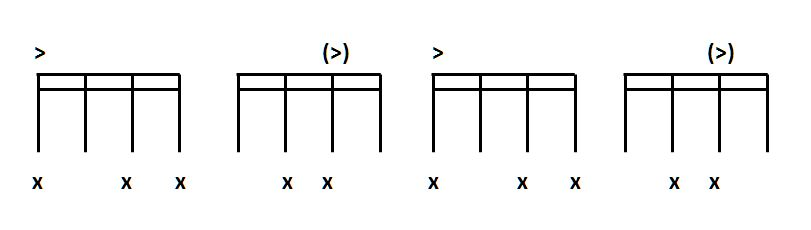
\includegraphics[width=0.9\linewidth]{kuvat/han1}\\
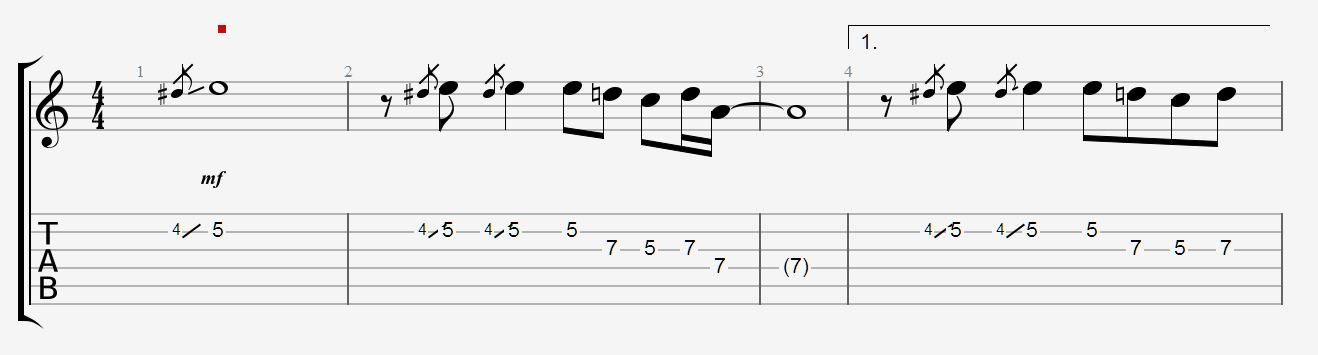
\includegraphics[width=0.9\linewidth]{kuvat/han2}\\
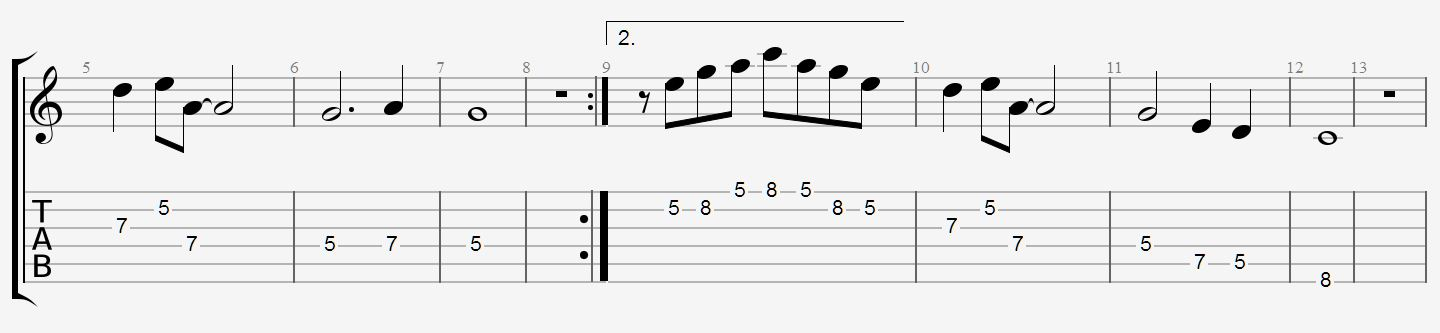
\includegraphics[width=0.9\linewidth]{kuvat/han3}\\
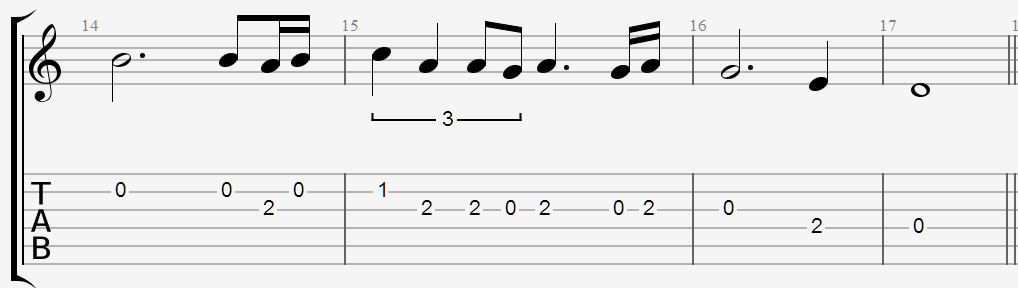
\includegraphics[width=0.9\linewidth]{kuvat/han4}

\endsong
		\addcontentsline{toc}{section}{\arabic{songnum} Missä muruseni on}
\beginsong{Missä muruseni on}[by={san. Mariska säv. Jenni Vartiainen, Jukka Immonen},
index={Yöllä taas mä meniin parvekkeelle nukkumaan}
]


% TAHTILAJI TÄHÄN:
\meter{12}{8}


%********** INTRO **********
\ifchorded
\beginverse*
{\nolyrics
|\[Am] |\[Am]
}
\endverse
\fi


%------------------------------------------------------------------------------
\beginverse\memorize[verse_oma]
%\musicnote{A}
|\[Am]Yöllä taas mä menin parvek|\[C]keelle nukkumaan,
|\[D]jotta lähempänä mua ois |\[F]hän.
|\[C]Pediltäni \[Em]taivas näkyy, |\[D]ryhdyin oottamaan,
|\[Am]että näen \[Em]tähden lentä|\[Am]vän.
\vspace{\versesep}
\replay[verse_oma]
|^Sanovat jos jossain huomaa |^tähdenlennon, niin
|^toivoa voit silloin mitä |^vaan.
|^Yöllä ylös ^taivaalle mä |^pyynnön kuiskasin:
|^Kävisipä ^pian tuule|^maan. \[Em/G]Tuuli,
\endverse

\beginchorus\memorize[chorus_oma]
|\[F]tuule sinne, missä |\[C]muruseni on,
|\[Em]leiki hetki hänen hiuksil|\[Am]laan. \[Em/G]Kerro
|\[F]rakkauteni, kerro |\[C]kuinka ikävöin.
|\[Em]Kerro, häntä ootan yhä va|\[Am]an. |\[Am]
\endchorus

%------------------------------------------------------------------------------
\beginverse\replay[verse_oma]
|^Tyyni oli eilen yö, mut |^kohta kuitenkin
|^tuuli henkäisi ja tuntee |^sain:
|^joku liikkui ^lähelläni, |^koski poskeain,
|^tutun käden ^tunsin ihol|^lain.
\vspace{\versesep}
\replay[verse_oma]
|^Enkä enää epäillyt, vaan |^tiesin, että voin
|^Niin kuin pieni lapsi nukah|^taa.
|^Ilma, jota ^hengitämme |^samaa ilmaa on ja
|^jalkojemme ^alla sama |^maa. \[Em/G]Tuuli,
\endverse

\beginchorus\memorize[chorus_oma]
|\[F]tuule sinne, missä |\[C]muruseni on,
|\[Em]leiki hetki hänen hiuksil|\[Am]laan. \[Em/G]Kerro 
|\[F]rakkauteni, kerro |\[C]kuinka ikävöin.
|\[Em]Kerro, häntä ootan yhä va|\[Am]an. \[Em/G]Tuuli

\vspace{\versesep}

|\[F]tuule sinne, missä |\[C]muruseni on,
|\[Em]leiki hetki hänen hiuksil|\[Am]laan. \[Em/G]Kerro 
|\[F]rakkauteni, kerro |\[C]kuinka ikävöin.
|\[Em]Kerro, häntä ootan yhä va|\[Am]an. \[Em/G]Tuuli

\vspace{\versesep}

|\[F]tuule sinne missä |\[C]muruseni o|\[Em]n.
|\[Am] \[Em/G] |\[F] |\[C] |\[Em]
|\[Am] |\[Am] |\[Amsus2]
\endchorus

%********** KITARAOTTEET **********
% Joitain otteita on tallennettuna kansioon "soinnut".
% Lisää voi tehdä itse käskyllä \gtab{}{}.
\ifchorded
\vspace{\versesep} % Tämä rivi luo välin kappaleen ja sointuotteiden väliin.
\noindent % Ei sisennystä.
\gtab{Am}{1:X02210:002310}
\gtab{C}{1:X32010:032010}
\gtab{D}{1:XX0232:000231}
\gtab{F}{1:133211:134211}
\gtab{Em}{1:022000:023000}
\gtab{Em/G}{1:322000:312000}
\gtab{Amsus2}{1:X02200:002300}
\fi

\endsong

        \addcontentsline{toc}{section}{\arabic{songnum} Luoksesi Tukholmaan}
\beginsong{Luoksesi Tukholmaan}[by={Säv. ja san.},
index={Taas aallot vaahtopäät laivaa kuljettaa}
]

\beginverse\memorize[verse_oma]
\[G] Taas aallot vaahtopäät laivaa \[Am]kuljettaa,
\[D7] yli aavan näin kohti \[G]Tukholmaa.
\[G] Näin vaiti seison luona \[Am]reelingin,
\[D7] kauas katselen miettein \[G]odottavin.
\endverse

\beginchorus\replay[verse_oma]
^ Näin saavun vihdoin luoksesi ^Tukholmaan,
^ jälkeen vuosien sinut ^nähdä saan.
^ Kauan jo päivää tätä ^kaipasin,
^ luoksein saapumaan oot valmis ^vihdoinkin.
\endchorus

\beginverse\replay[verse_oma]
^ Sä minut jätit vuonna ^seiskytviis,
^ Ruotsiin lähdit uskoen vain ^unelmiis.
^ Yksin tänne Helsinkiin mä ^silloin jäin,
^ joka ainut yö vain unta ^sinusta näin.
\endverse

\beginchorus\replay[verse_oma]
^ Näin saavun vihdoin luoksesi ^Tukholmaan,
^ jälkeen vuosien sinut ^nähdä saan.
^ Kauan jo päivää tätä ^kaipasin.
^ Luoksein saapumaan oot valmis ^vihdoinkin.
\endchorus

\beginverse\replay[verse_oma]
^ Sain eilen kirjees, jossa ^kerroit sen:
^ oli tullut aika kaipuun ^kyynelten.
^ Kovin kauan miettinyt mä ^silloin en,
^ nyt saavun luokses sua niin ^odottaen.
\endverse

\beginchorus\replay[verse_oma]
^ Näin saavun vihdoin luoksesi ^Tukholmaan,
^ jälkeen vuosien sinut ^nähdä saan.
^ Kauan jo päivää tätä ^kaipasin.
^ luoksein saapumaan oot valmis ^vihdoinkin.
\[D7] luoksein saapumaan oot valmis \[G]vihdoinkin.
\endchorus

\endsong
        \addcontentsline{toc}{section}{\arabic{songnum} Kaksi puuta}
\beginsong{Kaksi puuta}[
by={säv. ja san. Juha Tapio},
index={Minä rakastan näitä iltojani kanssas sun}
]

\meter{4}{4}

\ifchorded
\beginverse*
{\nolyrics
|\[Dm] |\[B&] |\[F] |\[C]
|\[Dm] |\[B&] |\[F] |\[F]
}
\endverse
\fi

\beginverse\memorize[verse_oma]
\musicnote{A}
|\[F] Minä rakastan näi|\[Am]tä iltojani kanssans
|\[Dm]sun, kun hetken päässä |\[B&]aamu odottaa.

|\[F] Ja me nauramme ja |\[Am]silmiämme pyyhimme, ja
|\[Dm]helppo huominen on unohta|\[B&]a.

|\[B&] Oomme taas kuin kaksi las|\[C]ta, ne jotka aikoi-
|\[Dm]naan puolivahingossa läh|\[C]ti samaa tietä kulkema|\[Dm]an.

Ja sä |\[B&]viet mut ikkunan lu|\[C]o
ja sä |\[B&]sanot: "Me kai ollaan niin kuin |\[C]nuo."
\endverse

\beginchorus\memorize[chorus_oma]
\musicnote{B}
|\[F] Kaksi vanhaa |\[C]puuta sateen pieksä-
|\[Dm]mää katsoo kevää|\[Am]seen, seisoo eril-
|\[B&]lään ja kestää joka |\[F/C]tuulen ja \[C]sään.

|\[F] Kaksi vanhaa |\[C]puuta, vaikket sitä
|\[Dm]nää, katsoo kevää|\[Am]seen, seisoo eril-
|\[B&]lään. Ja jossain alla |\[C7]maan ne kaiken aikaa 
|\[C7]yhteen punoneet on juuri-
\endchorus

\beginverse\replay[verse_oma]
\musicnote{A}
^aan. Kaksi ylvästä ja nu|^orta varmoina on voimis-
|^taan taivaan kantta |^kohti kasvaneet.

|^ Ehkä vuodet ovat |^kuorta ja talvet viimoil-
|^laan hiukan ohu|^emmaks raapineet.

|^ Kuinka onkaan kaksi |^lasta matkan myötä muuttune|^et
se ihme on kai |^vasta oomme tänne selvin|^neet.

Ja sä |^viet mut ikkunan lu|^o
ja sä |^sanot: "Mehän ollaan niin kuin |^nuo."
\endverse

\beginchorus\memorize[chorus_oma]
\musicnote{B}
|\[F] Kaksi vanhaa |\[C]puuta sateen pieksä-
|\[Dm]mää katsoo kevää|\[Am]seen, seisoo eril-
|\[B&]lään ja kestää joka |\[F/C]tuulen ja \[C]sään.

|\[F] Kaksi vanhaa |\[C]puuta, vaikket sitä
|\[Dm]nää, katsoo kevää|\[Am]seen, seisoo eril-
|\[B&]lään. Ja jossain alla |\[C7]maan ne kaiken aikaa 
|\[C7]yhteen punoneet on juuri-
\endchorus

\ifchorded
\beginverse*
{\nolyrics
\musicnote{C}
|\[Dm]aan. |\[B&] |\[F] |\[C]
|\[Dm] |\[B&] |\[F] |\[C]
}
\endverse
\fi

\beginchorus\memorize[chorus_oma]
\musicnote{B}
|\[F] Kaksi vanhaa |\[C]puuta sateen pieksä-
|\[Dm]mää katsoo kevää|\[Am]seen, seisoo eril-
|\[B&]lään ja kestää joka |\[F/C]tuulen ja \[C]sään.

|\[F] Kaksi vanhaa |\[C]puuta, vaikket sitä
|\[Dm]nää, katsoo kevää|\[Am]seen, seisoo eril-
|\[B&]lään. Ja jossain alla |\[C7]maan ne kaiken aikaa 
|\[C7]yhteen punoneet on juuri-

|\[F]aan. |\[F] |\[F] \[B&/F] |\[\Ferli{\bfseries\ttfamily F}]
\endchorus

\endsong
		\addcontentsline{toc}{section}{\arabic{songnum} Jos rakastat}
\beginsong{Jos rakastat}[by={san. Matti Rossi säv. Kai Chydenius},
index={Jos rakastat kylmää kuuta}
]

%% Säkeistöjen sisennys:
%\setlength{\versenumwidth}{0mm}

% TAHTILAJI
\meter{4}{4}


\beginverse*
\nolyrics \[A] \[A]
\endverse

\beginverse\memorize[verse_oma]
Jos \[A]rakastat kylmää \[A]kuuta,
\[A]esineitä, kirjojen \[A]kansia,
\[A]auton ovia, \[A7]ihmisen \[D]kuorta, \[D]
en \[Dm]tule sinun kanssasi \[Dm]meren rantaan,
\[A]enkä piirrä \[F#7]kuvaasi hiekkaan\ldots\[Hm] \[E7] \[A] \[A]
\endverse

\beginverse\replay[verse_oma]
Jos ^rakastat ikkun^oita
^hopeatuoppeja, ^soopeliturkkeja
^nahkaselkäistä ^vieras^kirjaa ^
minä ^hymyilen sinulle ^kadun poikki
mutta ^en lähde kanssasi ^hienoon paikkaan
^syömä^än hanhen^rintaa\ldots ^
\endverse

\beginverse\replay[verse_oma]
Jos ^rakastat purjehti^mista
^kaukomatkoja, ^Kanarian saarta
^pois sinä ^lähdet, ja minä pysyn ^täällä ^
Ja ^muistelen sinua ka^ipaamatta
^aamua, jolloin ^tuuli puhalsi
^hiuksissani, ja ^vei sinun ^kuvasi\ldots ^
\endverse

\beginverse\replay[verse_oma]
Jos ^rakastat setele^itä
minä ^autan sinua lu^opumaan niistä
ja ^annan sinulle ^kaiken, minkä ^tahdot, ^
mutta ^sydäntäni en ^anna\ldots ^ ^
^ ^ ^ ^
\endverse

\beginverse\replay[verse_oma]
Jos ^rakastat liikaa ^kirjoja
minä ^kysyn sinulta, ^miten käy minun
kun ^tunnet minut ^kannesta ^kanteen ^
ja ^juoneni lakkaavat ^kiinnostamasta
ja ^muistat ulkoa \[\Ferli{\bfseries\ttfamily F#7}]kaiken\ldots \[Hm] \[E7] \[A] \[A]
\endverse

\beginverse*
\nolyrics \[F7] \[F7]
\endverse

\beginverse
Jos \[B&]rakastat pieniä \[Gm]tyttöjä
\[E&]pieniä tyttöjä, \[F7]pieniä poikia
\[B&]koiria, mummoja, \[Gm]vanhojapiikoja
\[Cm7]salaattia ja \[F7]sellerinjuurta
\[B&]lampaanpaistia, \[D7]kevätaamuja,
\[E&]kylmien asemien \[G7]yksinäisiä \[Cm7]miehiä
minä \[F7]tulen sinun \[B&]kanssasi merenr\[F7]antaan
\endverse

\beginverse*
ja \[B&]pii\[D7]rrän, \[E&]piirrän kuvasi hi\[G7]ekkaan
ja \[Cm7]piirrän, \[F7]piirrän kuvasi hi\[B&]ekkaan. \[F7]
Ja \[B&]pii\[D7]rrän, \[E&]piirrän kuvasi hi\[G7]ekkaan
ja \[Cm7]piirrän, \[F7]piirrän kuvasi hi\[B&]ekkaan. \[E&] \[B&] \[B&]
\endverse

\endsong
		
		\addcontentsline{toc}{section}{\arabic{songnum} Kulkuri ja joutsen}
\beginsong{Kulkuri ja joutsen}[by={san. Reino Helismaa säv. Lasse Dahlquist},
index={Oon kulkuriksi syntynyt mä vainen}
]

%% Säkeistöjen sisennys:
\setlength{\versenumwidth}{0mm}

% TAHTILAJI
\meter{4}{4}

%********** 1. SÄKEISTÖ **********
% Säkeistön soinnut tallennetaan nimellä "verse_oma".
\beginverse\memorize[verse_oma]
Oon |\[C]kulkuriksi syntynyt mä |\[C]vainen
ja |\[C]paljain jaloin \[Em7]kierrän \[A7]maail|\[Dm7]maa. \[G7]
Näin |\[Dm7]kerran unta: joutsen taiva|\[G7]hainen
mun |\[Dm7]antoi hetken \[G7]kanssaan taival|\[C]taa.
Näin |\[C]maat ja metsät, järvet maani |\[C]armaan,
sen |\[Gm7]kaiken sini\[C7]taivahalta |\[F]näin. \[A7]
Tuuli |\[Dm7]lauloi laulu\[D#\(^\circ\)]jaan,
sadun |\[C]hohde \[B&7]peitti \[A7]maan,
\[A7]iha|\[Dm7]nampaa en mä \[G7]koskaan nähdä |\[G7-9]saa\[C]ta.
\endverse

%********** 2. SÄKEISTÖ **********
\beginverse\replay[verse_oma]
Ja |^laulun tämän lauloi mulle |^tuuli:
"On |^kaikkein kaunein ^aina ^oma |^maa. ^
Niin |^moni muuta paremmaksi |^luuli,
mut |^pettymyksen ^itsellensä |^saa.
Ei |^missään taivas sinisemmin |^loista,
ei |^missään hanki ^hohda kirkkaam|^min. ^
Tämä |^paina sydä^mees,
niin on |^taivas ^aina ^sees
^ja sun |^taipaleeltas ^murhe kauas |^kaik^koo."
\endverse   

%********** 3. SÄKEISTÖ **********
\beginverse\replay[verse_oma]
Niin |^päättyi uni, mutta vielä |^vuotan
mä |^kohtaavani ^kerran ^joutse|^nen, ^
ja |^siihen asti unelmiini |^luotan;
on |^helppo unek^sia ihmi|^sen.
Siks |^paljain jaloin onneani |^etsin
ja |^huolet laulu^llani haihdu|^tan. ^    
Elä|^mä on iha^naa,
kun sen |^oikein ^oival^taa
^ja kun |^lentää siivin ^valkein niin kuin |^jout^sen.
\endverse

\beginverse*
Elä|\[F]mä on iha\[\Ferli{\bfseries\ttfamily F}#\(^\circ\)]naa,        
kun sen |\[C]oikein \[B&7]oival\[\Ferli{\bfseries\ttfamily A7}]taa
ja kun |\[Dm7]lentää siivin \[G7]valkein niin kuin |\[\Ferli{\bfseries\ttfamily G7-9}]jout\[\Ferli{\bfseries\ttfamily C}]sen.
\endverse

%********** KITARAOTTEET **********
% Joitain otteita on tallennettuna kansioon "soinnut".
% Lisää voi tehdä itse käskyllä \gtab{}{}.
\ifchorded
%\vspace{\versesep} % Tämä rivi luo välin kappaleen ja sointuotteiden väliin.
%\noindent % Ei sisennystä.
%\gtab{Em}{1:022000:023000}
%\gtab{Am}{1:X02210:002310}
%\gtab{Am/F#}{1:202210:203410}
%\gtab{H7}{1:X21202:021304}
\fi


\endsong


%********** SEKALAISIA OHJEITA **********
%
%********** % **********
% Kaikki, mitä kirjoitetaan prosenttimerkin jälkeen
% samalle riville, jää kokonaan huomioitta lopulli-
% sessa dokumentissa.
%
%********** \brk **********
% \brk-käskyllä merkitään haluttu rivinvaihdon kohta.
% Jos rivi on liian pitkä lopullisessa dokumentissa,
% se katkeaa \brk:n kohdalta.
%
%********** \memorize[NIMI] **********
% Tallentaa soinnut tästä eteenpäin nimellä NIMI.
%
%********** \replay[NIMI] **********
% Ottaa NIMI-nimellä tallennetut soinnut käyttöön.
% Merkki ^ valisee seuraavan soinnun tallennetusta
% sointujonosta.
		
		\addcontentsline{toc}{section}{\arabic{songnum} Aikuinen nainen (kesken)}

\beginsong{Aikuinen nainen (kesken)}[by={suom. san. K. Liuhala säv. G. Savio--A. Gasalle},
index={Aikuinen nainen mä oon}
]

\meter{6}{8}


%-------------------------------------------------------------------------------
% INTRO
%-------------------------------------------------------------------------------
\beginverse*
|\[F] \[Fsus] |\[F] \[Fsus]
|\[F]Aikuinen \[Fsus]nainen mä oo|\[F]n, \[Fsus] 
|\[F]en enää eksy \[Dm]maailman |\[Gm]tuulii\[Gsus]n.
|\[Gm]Liittomme \[Gsus]vahvistukoo|\[Gm]n,
\[Bb]tahtoisin |\[F]jatkaa \[F]hyvin alkanutta |\[C]matkaa.
\endverse
%-------------------------------------------------------------------------------


%-------------------------------------------------------------------------------
% 1. SÄKEISTÖ
%-------------------------------------------------------------------------------
\beginverse
\[D7]Kun aika \memorize[verse_oma]|\[G]vaikeudet \[Gsus]tiellemme tu|\[G]o, \[Gsus]
|\[G]onnesta me teemme \[Em]suojaavan |\[Am]muuri\[Asus]n.
|\[Am]Voimaa tää \[Asus]rakkaus |\[Am]suo. \[C]Onnemme
|\[G]kestää, \[G]minkään emme anna |\[D]estää.
\[D]Paljosta lu|\[C]ovun, \[D7]jos saan luonain pitää
|\[G]sun. \[Em] |\[Am7] \[D7]
\endverse

\beginchorus\memorize[chorus_oma]
|\[G]E\[Em]|\[Am7]n \[D7]vapauttas tahdo
|\[G]riis\[Hm7]tä|\[Am7]ä, \[D7] tahdo
|\[G]e\[H7]n|\[Em] \[A7]itsenäisyyttäsi |\[Dsus]ki\[Dsus]is|\[D]tää.
\[D]Sua \[C]tar\[D7]vit|\[G]s\[G]e|\[C]n \[D7]sydänystäväksi
|\[G]ai\[H7]kuisen |\[Em]naisen.
\[C]Kaiken me |\[G]jaamme,
\[G]toisiamme tuke|\[D]kaamme.
\[D]Aikuinen |\[C]nainen \[D7]tuntee arvon rakkau|\[G]den. \[Gsus] |\[G] \[Gsus]
\endchorus
%-------------------------------------------------------------------------------

\beginverse\replay[verse_oma]
|^Selkääni käännä mä en
onnestani taistelen enkä pelkää
toisista huolehtien
kestämme paineet
meitä eivät kaada laineet
tuulilta suojaan sinut vien
jos viedä saan
\endverse

En vapauttas tahdo riistää
tahdo en itsenäisyyttäsi kiistää
sua tarvitsen sydänystäväksi
aikuisen naisen
kaiken me jaamme
toisiamme tukekaamme
aikuinen nainen tuntee arvon rakkauden

Sua tarvitsen sydänystäväksi
aikuisen naisen
kaiken me jaamme
toisiamme tukekaamme
aikuinen nainen tuntee arvon rakkauden.. (x2)


%********** 2. SÄKEISTÖ **********
% Säkeistön soinnut on tallennettuna nimellä "verse_oma".
% Ne otetaan käyttöön käskyllä \replay{}, ja ^-merkeillä.
%\beginverse\replay[verse_oma]
%Hän |^kuuntelee vain |^varjoja,
%ja |^nälkänsä hän ^unelmillaan \brk |^sammuttaa.
%\endverse

%********** 2. SÄKEISTÖN KERTOSÄE **********
%\beginchorus\replay[chorus_oma]
%Ja |^polte, joka ^sieluansa |^korven^taa,
%se on |^vain, ^vain rakka|^us. ^
%\endchorus

%********** KITARAOTTEET **********
% Joitain otteita on tallennettuna kansioon "soinnut".
% Lisää voi tehdä itse käskyllä \gtab{}{}.
\ifchorded
\vspace{\versesep} % Tämä rivi luo välin kappaleen ja sointuotteiden väliin.
\noindent % Ei sisennystä.
\gtab{F}{1:133211:134211}
\gtab{Fsus4}{1:133311:123411}
\gtab{Dm}{1:XX0231:000231}
\gtab{Gm}{1:355333:134111}
\gtab{Gsus4}{1:355533:123411}
\gtab{Bb}{1:X13331:012341}
\gtab{C}{1:X32010:032010}
\gtab{D7}{1:XX0212:0000213}
\gtab{Am}{1:X02210:002310}
\gtab{Asus4}{1:X02230:002340}
\gtab{Em}{1:022000:023000}
\gtab{G}{1:320003:210003}
\gtab{Gsus4}{1:3X0013:300014}
\gtab{Am7}{1:X02010:002010}
\fi


\endsong


%********** SEKALAISIA OHJEITA **********
%
%********** % **********
% Kaikki, mitä kirjoitetaan prosenttimerkin jälkeen
% samalle riville, jää kokonaan huomioitta lopulli-
% sessa dokumentissa.
%
%********** \brk **********
% \brk-käskyllä merkitään haluttu rivinvaihdon kohta.
% Jos rivi on liian pitkä lopullisessa dokumentissa,
% se katkeaa \brk:n kohdalta.
%
%********** \memorize[NIMI] **********
% Tallentaa soinnut tästä eteenpäin nimellä NIMI.
%
%********** \replay[NIMI] **********
% Ottaa NIMI-nimellä tallennetut soinnut käyttöön.
% Merkki ^ valisee seuraavan soinnun tallennetusta
% sointujonosta.
        
		\addcontentsline{toc}{section}{\arabic{songnum} Vain rakkaus}
\beginsong{Vain rakkaus}[by={Tapio Piirainen, Pekka Marjanen},
index={Hän vaeltaa}
]

\ifchorded
\beginverse*
{\nolyrics |\[Em] \[Em/D] |\[Cmaj7] \[H7] \rep{2}}
\endverse
\fi

\beginverse\memorize[verse_oma]
Hän |\[Em]vaeltaa läpi |\[Am]kaupungin,
hän |\[Am/F#]silmin pimein \[H7]etsii, ei |\[Em]löydä vain.
Kun |\[Em]ruumiinsa on |\[Am]tulessa,
hän |\[D7]kekäleitä kasaa syliin|\[Gmaj7]sä.
\endverse

\beginchorus\memorize[chorus_oma]
Ja |\[Am/F#]polte, joka \[H7]sieluansa |\[Em]korven\[Em/D]taa,
se on |\[Cmaj7]vain, \[H7]vain rakka|\[Em]us. \[Em/D] 
Se on |\[Cmaj7]vain, \[H7]vain rakka|\[Em]us. \[Em/D]
\endchorus

% Välisoitto
\beginverse*
{\nolyrics%
|\[Cmaj7] \[H7]
|\[Em] \[Em/D] |\[Cmaj7] \[H7]}
\endverse

\beginverse\replay[verse_oma]
Hän |^kuuntelee vain |^varjoja,
ja |^nälkänsä hän ^unelmillaan |^sammuttaa.
Jos |^kaipaus on |^myrkkyä,
hän |^pimeydestä siihen sukel|^taa.
\endverse

\beginchorus\replay[chorus_oma]
Ja |^polte, joka ^sieluansa |^korven^taa,
se on |^vain, ^vain rakka|^us. ^ 
Se on |^vain, ^vain rakka|^us. ^
\endchorus

\beginverse*
{\nolyrics%
|\[Cmaj7] \[H7]
|\[Em] \[Em/D] |\[Cmaj7] \[H7]}
\endverse

\beginverse\replay[verse_oma]
Hän |^tähtiyötä |^katselee
ja |^kuulee näkee ^kaiken, minkä |^nähdä voi.
Kun |^hiljaisuus on |^erämaa,
se |^mykän huudon jostain parkai|^see.
\endverse

\beginchorus\replay[chorus_oma]
Ja |^polte, joka ^sieluansa |^korven^taa,
se on |^vain, ^vain rakka|^us. ^ 
Se on |^vain, ^vain rakka|^us. ^
Se on |\[Cmaj7]vain, \[H7]vain rakka|\[Emadd9]us.
\endchorus

\ifchorded
\vspace{10mm}
\noindent
\gtab{Am}{1:X02210:002310}
\gtab{Am/F#}{1:202210:203410}
\gtab{H7}{1:X21202:021304}
\gtab{Cmaj7}{1:X32000:023000}
\gtab{D7}{1:XX0212:0000213}
\gtab{Em}{1:022000:023000}
\gtab{Em/D}{1:XX0000:000000}
\gtab{Emadd9}{1:024000:013000}
\gtab{Gmaj7}{1:320002:320001}
\fi

 \endsong
		\addcontentsline{toc}{section}{\arabic{songnum} Syyslaulu}
\beginsong{Syyslaulu}[by={Tove Jansson, Erna Tauro},
%cr={\copyright },
index={Kiirehdi rakkain}
%,li={\today}
]

\beginverse\memorize[verse_oma]
\musicnote{A1}
|\[Em]Kotimatka pitkä niin, ei |\[Em]vastaantuli\[F#]jaa,
illat |\[Am]sammuvat \[H7]kylmään hämä|\[Em]ryyteen.
Jo |\[Em]tule lohduttamaan, synkkä |\[Em]mieli pujah\[F#]taa
syksy|\[Am]iltani \[H7]yksinäi|\[Em]syyteen.
\musicnote{A2}
Kas, |\[Am]pimeähän saa sitä |\[Em]ajattelemaan,
mitä |\[Am]muuten ei \[D7]muistaisi |\[G]lainkaan.
Nyt |\[Am]muistan miten paljon mä |\[Em]tehdä tahdoin\[C7]kaan,
miten |\[H7]vähän siitä aikaan mä |\[Em]sain\[D7]kaan.
\endverse

\beginchorus\memorize[chorus_oma]
\musicnote{B}
|\[G]Kiirehdi \[Hm]rakkain, jos |\[C]rakkaus \[Am]kutsuu.
|\[D7]Päivän ei hetket niin |\[G]pit\[B&\(^\circ\)]kiä \[D7]lie. \[D7]
|\[G]Suo valon \[Hm]syttyä, |\[C]yö kohta \[Am]saapuu.
|\[D7]Pois kesän kukkaset |\[D7]syk\[Am]sy \[H7]vie. \[H7]
\endchorus

\beginverse\replay[verse_oma]
\musicnote{A1}
|^Etsin jotain, mikä meiltä |^unohtunut ^on,
minkä |^löytää mä ^avullasi |^voisin.
On |^kesä lyhyt niin kuin haave |^saavuttama^ton
siitä, |^mikä oisi ^voinut olla |^toisin.
\musicnote{A2}
Kai |^tulet pian ennen kuin |^pimeään mä jään,
eihän |^kaikki kai ^ole mennyt |^hukkaan.
Jos |^löytäisimme toisemme, |^silloin ehkä ^nään
keinon, |^jolla vielä kaiken saamme |^kuk^kaan.
\endverse

\beginchorus\replay[chorus_oma]
\musicnote{B}
|^Kiirehdi ^rakkain, jos |^rakkaus ^kutsuu.
|^Päivän ei hetket niin |^pit^kiä ^lie. ^
|^Suo valon ^syttyä, |^yö kohta ^saapuu.
|^Pois kesän kukkaset |^syk^sy ^vie. ^
\endchorus

\beginverse\replay[verse_oma]
\musicnote{A1}
|^Syksyn tuuli mukanaan vie |^kesän muistot^kin,
nyt jo |^turhaan sä ^kysyt, minne |^vie tää.
Nyt |^rakastan kai vähemmän kuin |^ennen rakas^tin,
mutta |^enemmän kuin ^koskaan saat |^tietää.
\musicnote{A2}
Nyt |^majakat me näämme, kun |^myrsky raivoaa,
tuuli |^vaahtopäiden ^äänen tänne |^kantaa.
Ja |^tärkeintä on sydämmemme |^ääntä ^noudattaa
ja |^kaikkemme toisillemme |^an^taa.
\endverse

\beginchorus\replay[chorus_oma]
\musicnote{B}
\lrep ^Kiirehdi ^rakkain, jos |^rakkaus ^kutsuu.
|^Päivän ei hetket niin |^pit^kiä ^lie. ^
|^Suo valon ^syttyä, |^yö kohta ^saapuu.
|^Pois kesän kukkaset |^syk\[D7*]sy \[G]vie. \rrep
\endchorus

\ifchorded
\vspace{10mm}
\texttt{D7*} = \texttt{D7} vaihtobassolla
\vspace{10mm}
\noindent
\gtab{Am}{1:X02210:002310}
\gtab{Hm}{1:X24432:013421}
\gtab{H7}{1:X21202:021304}
\gtab{B&\(^\circ\)}{1:XX2323:001324}
\gtab{C}{1:X32010:032010}
\gtab{C7}{1:X32310:032410}
\gtab{D7}{1:XX0212:000213}
\gtab{D7*}{1:X00212:000213}
\gtab{Em}{1:022000:023000}
\gtab{F#}{1:244322:134211}
\gtab{G}{1:320003:210003}
\fi

\endsong
		
        
        %\ifchorded\scleardpage\fi % Seuraava laulu alkaa parittoman sivun alusta.
        \addcontentsline{toc}{section}{\arabic{songnum} Tähdet tähdet}
\beginsong{Tähdet, tähdet}[by={Säv. ja san. Rauli Somerjoki},
index={Saapunut luokseni yö on}
]

\beginverse\memorize[verse_oma]
|\[Am]Saapunut luokseni |\[G]yö on,
|\[Am]silmäni luon taivaa|\[E7]seen.
|\[F]Tumma se katto |\[Dm]tähtinä tuikkii,
on |\[F]katseensa tutkima|\[E7]ton.
|\[Am]Suunnaton tähtien |\[G]määrä
|\[Am]häipyen kaukaisuu|\[E7]teen.
|\[F]Niin pientä rataa |\[Dm]maapallo makaa
|\[H7]omaansa ain uudel|\[E7]leen. |\[E7]
\endverse

\beginchorus\memorize[chorus_oma]
Tähdet, |\[Am]tähdet, |\[Am]luoksenne tahtoisin |\[Dm]pois.
|\[Dm] Tähdet, |\[E7]tähdet, |\[E7]silloin mun helpompi |\[Am]ois.
|\[D] \[E7]Tähdet, |\[Am]tähdet, |\[Am]enkö jo tulla mä |\[Dm]saa,
tähdet, |\[E7]tähdet, |\[E7]ikuisuuksiin ajan |\[Am]taa? |\[E7]
\endchorus

\beginverse\replay[verse_oma]
|^Turha on toiveita |^kantaa,
|^turha on haaveiden |^tie.
|^Jos jotain antaa |^tai lemmenrantaa
käy |^santaan, se suoraan vain |^vie.
|^Aamuhun yön tähdet |^haipuu,
|^idässä pian ruskot|^taa.
|^Karvas jää kaipuu, |^pää alas taipuu,
|^päivä käy uus koitta|^maan. |^
\endverse

\beginchorus\replay[chorus_oma]
Tähdet, |^tähdet, |^luoksenne tahtoisin |^pois.
|^ Tähdet, |^tähdet, |^silloin mun helpompi |^ois.
|^ ^Tähdet, |^tähdet, |^enkö jo tulla mä |^saa,
tähdet, |^tähdet, |^ikuisuuksiin ajan |^taa? |^
\endchorus

\beginchorus\replay[chorus_oma]
Tähdet, |^tähdet, |^luoksenne tahtoisin |^pois.
|^ Tähdet, |^tähdet, |^silloin mun helpompi |^ois.
|^ ^Tähdet, |^tähdet, |^enkö jo tulla mä |^saa,
tähdet, |^tähdet, |^ikuisuuksiin ajan |^taa? |\[Am] \[Am9]
\endchorus

\endsong
        \addcontentsline{toc}{section}{\arabic{songnum} Valot}
\beginsong{Valot}[by={Rauli Somerjoki},
index={Ilta saapuu hiljaa huoahtain}
]

\capo{2}

\meter{12}{8}

\ifchorded
\beginverse*
{\nolyrics |\[Am] \[D7] |\[G] \[G]}
\endverse
\fi

\beginverse\memorize[verse_oma]
|\[G]Ilta saapuu \[Em]hiljaa huoah|\[H7]tain,
|\[C]valot syttyy \[Am7]taakse i\[D7]kku- \brk |\[Gmaj7]nain. \[Gmaj7] \[G6] \[Hm7]
Ei |\[Am7]jää yksi\[D7]nään muut, |\[G]kukaan pimeään,
|\[Em]valot pois yön \[A7]varjot häivyt|\[D7]tää.

\vspace{\versesep}

Vaan, |\[G]vaan mä niitä \[Em]sytytäkkään |\[H7]en,
|\[C]luulen, tuskin \[Am7]niitä \[D7] tarvit- \brk |\[Gmaj7]sen, \[Gmaj7] \[G6] \[Hm7]
|\[Am7]kun sinä \[D7]niin olet |\[H7]valo kirkka\[C]hin.
Sanoi|\[A7]sin, liikaa\[D7]kin se valai|\[G]see.
\endverse

\beginverse\replay[verse_oma]
|^Kaikki tahtoo ^tietää, miksi |^jää
|^asuntoni ^aivan ^ pime- \brk |^ään. ^ ^ ^
|^Varjot kietou^tuu, |^niihin tukehtuu,
|^mulle vaikka ^mitä tapah|^tuu.

\vspace{\versesep}

Vaan |^ne ei tiedä, ^että valo |^vois
|^säikyttää tän ^aran ^ tunteen \brk |^pois. ^ ^ ^
|^Siis kahdes^taan päätet|^tiin: ei milloin^kaan
valot |^käy meitä ^päin pala|^maan
\endverse

\ifchorded
\vspace{\versesep}
\noindent
\gtab{C}{1:X32010:032010}
\gtab{D7}{1:XX0212:0000213}
\gtab{Em}{1:022000:023000}
\gtab{G}{1:320003:210003}
\gtab{Gmaj7}{1:320002:320001}
\gtab{G6}{1:320000:320000}
\gtab{Am}{1:X02210:002310}
\gtab{Am7}{1:X02010:002010}
\gtab{H7}{1:X21202:021304}
\gtab{H7}{1:X23232:013121}
\gtab{Hm7}{1:X24232:013121}
\fi

\endsong
        
        \begin{intersong}
        	\centering
        	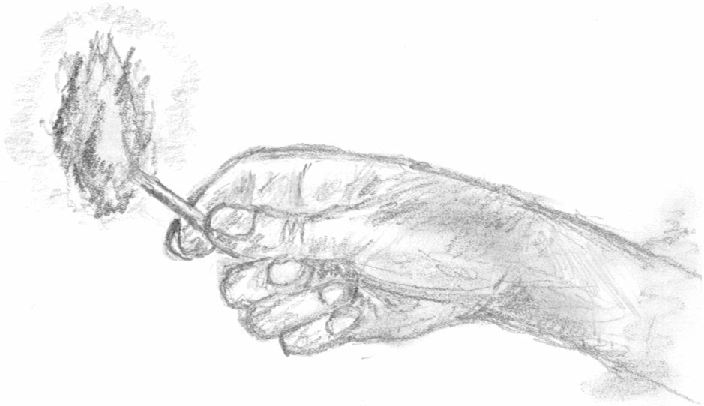
\includegraphics[width=0.5\linewidth]{kuvat/valot}
        \end{intersong}
        
        %\ifchorded\scleardpage\fi % Seuraava laulu alkaa parittoman sivun alusta.
        \addcontentsline{toc}{section}{\arabic{songnum} Marilyn}
\beginsong{Marilyn}[by={Säv. ja san. Juice Leskinen},
index={Mä taivalsin läpi tuulen ja tuiskun}
]

\beginverse\memorize[verse_oma]
\musicnote{A}
Mä |\[C]taivalsin \[Am]läpi |\[F]tuulen ja \[G7]tuiskun
|\[C]nähdäk\[Am]seni sun |\[F]puuteri\[G7]huiskun.
Mä |\[C]silmäni \[Am]suljin ja |\[F]sinut näin \[G7]tytössä
|\[C]naapurin. \[Am] |\[F] \[G7]

Olin |\[C]nuori ja \[Am]keuhkoissa |\[F]kirveli \[G7]Boston.
|\[C]Brylcreemi\[Am]kutreilla |\[F]keikkui \[G7]Roston.
Sä |\[C]olit mun \[Am]nainen, |\[F] nainen, \[G7]Mari|\[C]lyn. |\[C7]

\musicnote{B}
Mä |\[F]tuijottelin |\[F]silloin vain |\[C]sinun herkku|\[C]poveen
ja |\[D7]kuuta ulvoin |\[F]illoin
|\[G7\tiny tacet I] langenneena |\[G7\tiny tacet I]loveen! (Ja mä lauloin:)
\endverse

\beginchorus\memorize[chorus_oma]
\musicnote{C}
|\[F] Marilyn, |\[C]Marilyn! |\[G7]Milloin riisut |\[C]jumpperin?
|\[F] Marilyn, |\[C]Marilyn! Tuon
|\[G7\tiny tacet II]ajan (tuon ajan, tuon \brk |\[G7\tiny tacet II]ajan) saanko koskaan takai-
|\[C]sin? \[Am] |\[F] \[G7]
|\[C] \[Am] |\[F] \[G7]
\endchorus

\beginverse\replay[verse_oma]
\musicnote{A}
Mä |^tuli^sesti sua |^kirjeillä ^lemmin
vaikka |^MGM ^vastaili |^viralli^semmin
Mua |^mitkään ^voimat |^silloin masen^taneet
|^ei ^ |^ ^

Mä |^rahani ^tuhlasin |^sun joka ^leffaan
ja |^unessa ^hampaat |^iskin sun ^peffaan
Oli |^kaikkein ^pyhin |^sinun ^hurlum|^hei |^

\musicnote{B}
Ja |^kun sun nurin|^niskoin sai |^kirjailija |^Arttu
mä |^seinältä sun |^kiskoin,
|^ sä olit pelkkä |^narttu (ja mä lauloin)
\endverse

\beginchorus\replay[chorus_oma]
\musicnote{C}
|^ Marilyn, |^Marilyn! |^Milloin riisut |^jumpperin?
|^ Marilyn, |^Marilyn! Tuon
|^ajan (tuon ajan, tuon \brk |^ajan) saanko koskaan takai-
|^sin? ^ |^ ^
|^ ^ |^ ^
\endchorus

\beginverse\replay[verse_oma]
\musicnote{A}
Sun |^kuvasi ^kanssa mä |^sänkyyn ^hiivin
ja |^siitä Holly^woodiin |^aatosten ^siivin
Mä |^itseni ^uneen |^itkin ja ^uniin
|^onanoin ^ |^ ^

Mä |^jengissä ^näyttelin |^kovaa ^jätkää
muut |^jumaloi ^mua ja |^minun ^prätkää
Muut |^jumaloi ^mua, mä |^sinua ^juma-
|^loin |^ (ja mä lauloin)
\endverse

\beginchorus\replay[chorus_oma]
\musicnote{C}
|^ Marilyn, |^Marilyn! |^Milloin riisut |^jumpperin?
|^ Marilyn, |^Marilyn! Tuon
|^ajan (tuon ajan, tuon \brk |^ajan) saanko koskaan takai-
|\[F]sin? Marilyn, |\[C]Marilyn! |\[G7]Milloin palaat |\[C]takaisin?
|\[F] Marilyn, |\[C]Marilyn! |\[G7\tiny tacket I] Täällä ootan |\[G7\tiny tacket I]kanssa jumppe|\[C]rin!
|\[C] Shoobido!
\endchorus

\ifchorded
\vspace{5mm}
\noindent
\gtab{C}{1:X32010:032010}
\gtab{Am}{1:X02210:002310}
\gtab{F}{1:133211:134211}
\gtab{G7}{1:320001:320001}
\newline
\gtab{C7}{1:X32310:032410}
\gtab{D7}{1:XX0212:0000213}
\gtab{G7}{1:320001:320001}
\fi

\endsong
        
        %\ifchorded\scleardpage\fi % Seuraava laulu alkaa parittoman sivun alusta.
        \addcontentsline{toc}{section}{\arabic{songnum} Tahroja paperilla}
\beginsong{Tahroja paperilla}[by={Matti Syrjä, Mikko Syrjä},
index={Tiedän että on yö}
]

\ifchorded
\beginverse*
{\nolyrics |\[Am] |\[Am] |\[Am] |\[Am]}
\endverse
\fi

\beginverse\memorize[verse_oma]
\musicnote{A}
|\[Am] Tiedän että on y|\[D]ö,
|\[H] kun saavut kotiisi |\[E7]pimeään.
|\[Am] Yksinäisyys ly|\[D]ö
|\[H] sanomatta ni|\[E7]meään.
|\[F] Kun luet \[G]kirjeeni, |\[C]kaiun k\[Am]uulet,
|\[F]tahrat näet, |\[E7]joita sateeksi |\[Am]luulet. |\[Am]

\vspace{\versesep}

\replay[verse_oma]
|^ Kuljen ulkona va|^lossa,
|^kasvoillani voin |^tuntea tuulen.
|^ Ei sitä tuntunut ta|^lossa,
|^ johon palaa en |^koskaan, luulen.
|^ En ole ^menossa |^minnekk^ään.
Ei |^missään tulee |\[F]minun luokse- \brk n|\[E7]i, minun |\[E7]vuokseni.
\endverse

\beginchorus\memorize[chorus_oma]
\musicnote{B}
Vain |\[F]tahroja paperilla, |\[G]älä siis suutu,
ei |\[C]niistä asiat |\[Am]miksikään muutu.
Ei |\[F]se että meillä oli |\[E7]retkemme,
eikä |\[Am]se että meillä oli |\[G]hetkemme.
Voi |\[F]tuuli kylmästi |\[G]kutittaa selkää,
se |\[C]eteenpäin työntää, |\[Am]älä siis pelkää.
Älä |\[F]huoli siitä, sillä |\[E7]meillä oli hetkem|\[Am]me. A-a|\[G]a,
|\[F]muista, että |\[E7]meillä oli |\[E7] hetkemme. |\[Am] |\[Am]
\endchorus

\beginverse\replay[verse_oma]
\musicnote{A}
|^ Kutsun saaneena tu|^lin,
|^lähdin kuin varas, |^säikähdin. Viimein
|^ kun itseeni ta|^rttuneen
|^tajusin va|^rttuneen.
|^Imin sut ku^iviin, |^tarttui mun hu^iviin
|^tuoksusi, teit |\[F]saman minulle.
|\[E7]Juoksusi annan |\[E7]anteeksi sinulle.
\endverse

\beginchorus\replay[chorus_oma]
\musicnote{B}
Vain |^tahroja paperilla, |^älä siis suutu,
ei |^niistä asiat |^miksikään muutu.
Ei |^se että meillä oli |^retkemme,
eikä |^se että meillä oli |^hetkemme.
Voi |^tuuli kylmästi |^kutittaa selkää,
se |^eteenpäin työntää, |^älä siis pelkää.
Älä |^huoli siitä, sillä |^meillä oli hetkem|^me. A-a|^a,
\endchorus

\beginchorus\replay[chorus_oma]
Vain |^tahroja paperilla, |^älä siis suutu,
ei |^niistä asiat |^miksikään muutu.
Ei |^se että meillä oli |^retkemme,
eikä |^se että meillä oli |^hetkemme.
Voi |^tuuli kylmästi |^kutittaa selkää,
se |^eteenpäin työntää, |^älä siis pelkää.
Älä |^huoli siitä, sillä |^meillä oli hetkem|^me. A-a|^a,
|^muista, että |^meillä oli |^ hetkem|^me. |\[Asus2]
\endchorus

\ifchorded
\vspace{\versesep}
\noindent
\gtab{C}{1:X32010:032010}
\gtab{D}{1:XX0232:000231}
\gtab{E7}{1:020100:020100}
\gtab{F}{1:133211:134211}
\gtab{G}{1:320003:210003}
\gtab{Am}{1:X02210:002310}
\gtab{Asus2}{1:X02200:002300}
\gtab{H}{1:X24442:012341}
\fi

\endsong
        
        %\ifchorded\scleardpage\fi % Seuraava laulu alkaa parittoman sivun alusta.
        
        \addcontentsline{toc}{section}{\arabic{songnum} Ranskalaiset korot}
\beginsong{Ranskalaiset korot}[by={Erik Lindström, Hillevi},
index={Näin sävel soi askelten}
]

\beginverse
\memorize[verse_oma]
\musicnote{A}
	Näin sävel |\[F7]soi \[E7]askel|\[Am]ten,
	ja ikku|\[F7]nassaan poika jo on. |\[E7]
	Taas kato|\[F7]aa \[E7]neitonen |\[Am]
	- on poika |\[F7]yksin \[E7] ja rauha|\[Am]ton.
\replay[verse_oma]
\musicnote{A}
	Niin tuttu |^on ^ääni tuo |^
	sen joka |^päivä kuulla hän |^saa;
	ei öisin|^kään ^rauhaa |^suo,
	ja unis|^saankin ^ hän odot|^taa.
\endverse

\beginchorus
\memorize[chorus_oma]
\musicnote{B}
	Hän |\[Dm6]toivoo, että \[E7]edes yhden |\[Am]kerran
	nuo |\[Dm6]ranskalaiset \[E7]korot seisah|\[Am]tais
	ja |\[Dm6]että edes \[E7]pienen hetken |\[Am]verran
	tuon |\[F7]tytön nähdä hän |\[E7]sais.
\endchorus
\beginverse*
\replay[verse_oma]
\musicnote{A}
	Näin sävel |^soi ^askel|^ten.
	Se ainut |^laulu pojalle |^on.
	Oi, missä |^on ^tyttö sen? |^
	On pojan |^sydän ^ niin rauha|^ton.
\endverse

% 2. säkeistö

\beginverse
\replay[verse_oma]
\musicnote{A}
	Näin sävel |^soi ^askel|^ten,
	ja ikku|^nassaan poika jo on. |^
	Taas kato|^aa ^neitonen |^
	- on poika |^yksin ^ ja rauha|^ton.
\replay[verse_oma]
\musicnote{A}
	Niin tuttu |^on ^ääni tuo |^
	sen joka |^päivä kuulla hän |^saa;
	ei öisin|^kään ^rauhaa |^suo,
	ja unis|^saankin ^ hän odot|^taa.
\endverse

\beginchorus
\replay[chorus_oma]
\musicnote{B}
	Niin |^kerran luona ^puiston portin|^pielen
	nuo |^askeleet hän ^kuuli yllät|^täin.
	Hän |^taisi yhden ^sanan ranskan |^kielen:
	Che|^ri, hän kuiskasi |^näin.
\endchorus
\beginverse*
\replay[verse_oma]
\musicnote{A}
	Taas sävel |^soi ^askel|^ten,
	mut yhä |^kiinni ikkuna |^jää.
	Vie poika |^pois ^tyttösen|^
	ja tytöl|^lensä ^ näin vihel|^tää,
	(viheltäen) |\[F7] \[E7] |\[Am]
%	ja tytöl|\[F7]lensä \[E7] näin vihel|\[Am]tää,
	ja tytöl|\[F7]lensä \[E7] näin vihel|\[Am6]tää.
\endverse

\ifchorded
\vspace{10mm}
\noindent
\gtab{Am}{1:X02210:002310}
\gtab{Am6}{1:X02212:002314}
\gtab{Dm6}{1:XX0201:000201}
\gtab{E7}{1:020100:020100}
\gtab{F7}{1:131211:131211}
\fi

\endsong
        \addcontentsline{toc}{section}{\arabic{songnum} Jos sä tahdot niin}
\beginsong{Jos sä tahdot niin}[by={Hector},
%cr={\copyright },
index={Jos sä tahdot niin}
%,li={\today}
]

\beginverse*
\nolyrics |\[G/D] \[G/D] \[Gsus4/D\tiny(koru)] \[G/D]
|\[C/E] \[C/E] \[C7/F\tiny(koru)] \[C/E]
|\[G/D] \[G/D] \[Gsus4/D\tiny(koru)] \[G/D]
\endverse

\beginverse\memorize[verse_oma]
|\[^C/E\tiny(murto alas)] Jos sä tahdot |\[G]niin, \[G] olen
|\[G]sulle joku \[G] aivan |\[C\tiny(koru)]muu. |\[^G]
%
|\[C] Jos sä \[C]tahdot |\[G]niin, \[G] olen
|\[Dm]virhe, joita \[Dm]tapah|\[Am]tuu. \[Am]
Jos sä |\[F]tahdot niin, \[F] tulen |\[G]jouluksi \[G]kotiin.
Jos sä |\[Am]tahdot niin, \[Am] en enää |\[F]lähde uusiin \[F]sotiin.
Jos sä |\[G]tahdot niin, \[G] jään vahti|\[Dm]koiraksi \[Dm]ovel|\[Am]les \[Am]
tai painan |\[Dm]pääni sun \[Dm] povel|\[Am]les... |\[G]
\endverse

\beginverse*\replay[verse_oma]
|\[C\tiny(murto alas)] Jos sä tahdot |^niin ^– et enää
|^koskaan ole ^ levo|^ton. |\[G/D] \[G/D] \[Gsus4/D] \[G/D]
%
|^ Jos sä ^tahdot |^niin ^- kaikki
|^minun myöskin ^- sinun |^on. ^
Jos sä |^tahdot niin, ^ otan |^sinun uskon^tosi.
Jos sä |^tahdot niin, ^ on mulle |^valheesikin ^tosi.
Jos sä |^tahdot niin, ^ muutan |^kirjoille ^Andor|^raan, ^
jos vielä |^siellä sut ^nähdä |^saan,
\endverse

\beginchorus\memorize[chorus_oma]
sillä |\[F]ilman sinu\[F]a hukun |\[G]öihin seka\[G]viin
ja ilman |\[Am]sinua, \[Am] no |\[F]niin; \[F]
ilman |\[G]sinua, \[G] olen |\[Dm]puolitiessä \[Dm]helvet|\[Am]tiin... |\[G]
\endchorus

\beginverse\replay[verse_oma]
|\[C\tiny(murto alas)] Jos sä tahdot |^niin ^ nime|^äsi enää ^ toista |^en. |\[G/D] \[G/D] \[Gsus4/D] \[G/D]
|^ Mut vaikka ^tahdot |^niin ^– kuvaas |^mielestäni ^poista |^en. ^
Jos sä |^tahdot niin ^- tulen |^kallioiden ^läpi.
Jos sä |^tahdot niin ^– what |^ever makes you ^happy.
Jos sä |^tahdot niin ^– tuon sulle \brk |^Tiibetin ^vuotee|^seen. ^
tai siirrän |^pohjoisen ^luotee|^seen. \[Am]
ja aina |\[Dm]uudelleen ja \[Dm]uudel|\[Am]leen. \[Am]
sun muistan |\[Dm]joskus mua \[Dm]suudel|\[Am]leen... \[Am]
\endverse

\beginchorus\replay[chorus_oma]
Mutta |^ilman rakka^utta hukun |^öihin seka^viin
ja ilman |^rakkautta ^- no |^niin; ^
ilman |^rakkautta ^- olemme |^puolitiessä ^helvet|^tiin...
\endchorus

\beginverse*
|\[Dm] Jos sä \[Dm]tahdot |\[Am]niin \[Am]
|\[Dm] Jos sä \[Dm]tahdot |\[Am]niin \[Am]
|\[Dm6\tiny(murto alas)] Jos sä tahdot |\[Amadd9\tiny(murto alas)]niin
\endverse

\ifchorded
\vspace{\versesep} % Tämä rivi luo välin kappaleen ja sointuotteiden väliin.
\noindent % Ei sisennystä.
\gtab{G/D}{1:XX0003:000004}
\gtab{Gsus4/D}{1:XX0013:000014}
\gtab{C/E}{1:XX2013:002014}
\gtab{C7/F}{1:XX3013:003014}
\gtab{C}{1:X32013:032014}
\gtab{C"koru"=F}{1:XX3013:003014}
\gtab{D7sus4}{1:XX0201:000201}
\gtab{Amadd7}{1:X02500:001400}
\fi

\endsong

%\ifchorded\scleardpage\fi % Seuraava laulu alkaa parittoman sivun alusta.
\addcontentsline{toc}{section}{\arabic{songnum} Nopeimmat junat}
\beginsong{Nopeimmat junat}[by={Anna Puu},
index={Olen kasvanut kiinni maahan}
]

\capo{3}

% TAHTILAJI TÄHÄN:
\meter{4}{4}


%********** INTRO **********
\ifchorded
\beginverse*
{\nolyrics
|\[F] |\[G] |\[F] |\[G]
|\[F] |\[G] |\[C] |\[C]
}
\endverse
\fi


%********** 1. SÄKEISTÖ **********
% Säkeistön soinnut tallennetaan nimellä "verse_oma".
\beginverse\memorize[verse_oma]
|\[F] Olen kasvanut |\[G]kiinni maahan, \brk|\[F] lapsuuden |\[G]maisemaan.
|\[F] Olen kasvanut |\[G]kiinni poikaan,  \brk|\[C]siihen yhteen ja |\[Dm]oikeaan.
|\[F] Olen kasvanut |\[G]kiinni taloon, \brk|\[F] jonka ikkunan|\[G]pielistä vetää.
|\[F] En tahdo |\[G]kuuta taivaal|\[C]ta \brk kuin kerran |\[Dm]vuoteen |\[F]enää.
Paikka se on |\[G]tämäkin.
\endverse


%********** 1. SÄKEISTÖN KERTOSÄE **********
\beginchorus\memorize[chorus_oma]
|\[C] Pilvien |\[C]alla, maan |\[Dm]päällä, |\[Dm]
|\[Em] mutta nopeimmat |\[Em]junat eivät, \brk|\[F] pysähdy |\[G]enää täällä.
|\[C] Pilvien |\[C]alla, maan |\[Dm]päällä, |\[Dm]
mutta |\[F]nopeimmat \[Em]junat, |\[Dm]nopeimmat \[C]junat,
ei |\[Am]nopeimmat \[G]junat enää  \mbar{2}{4}\[F\tiny(1/2)]pysähdy  \mbar{4}{4}\[C]täällä. |\[C]
\endchorus

%********** INTERLUDE **********
\ifchorded
\beginverse*
{\nolyrics
|\[F] |\[G] |\[F] |\[G]
|\[F] |\[G] |\[C] |\[C]
}
\endverse
\fi

%********** 2. SÄKEISTÖ **********
% Säkeistön soinnut on tallennettuna nimellä "verse_oma".
% Ne otetaan käyttöön käskyllä \replay{}, ja ^-merkeillä.
\beginverse\replay[verse_oma]
|^ Olen kasvanut |^kiinni lähtöön, \brk|^ kaupungin |^kaipuuseen.
|^ Lähtenyt |^monta kertaa, \brk|^palannut aina |^entiseen.
|^ Olen kasvanut |^kiinni talveen, \brk|^ sen kuristus|^otteeseen
|^ Kun pysyn sun |^luonas tiedän, \brk|^vielä jaksan |^kevääseen
|^ Paikka se on |^tämäkin
\endverse

%********** 2. SÄKEISTÖN KERTOSÄE **********
\beginchorus\replay[chorus_oma]
|\[C] Pilvien |\[C]alla, maan |\[Dm]päällä, |\[Dm]
|\[Em] mutta nopeimmat |\[Em]junat eivät, \brk|\[F] pysähdy |\[G]enää täällä.
|\[C] Pilvien |\[C]alla, maan |\[Dm]päällä, |\[Dm]
mutta |\[F]nopeimmat \[Em]junat, |\[Dm]nopeimmat \[C]junat,
ei |\[Am]nopeimmat \[G]junat enää  \mbar{2}{4}\[F\tiny(1/2)]pysähdy  \mbar{4}{4}\[C]täällä. |\[C]
\endchorus

%********** INTERLUDE **********
\ifchorded
\beginverse*
{\nolyrics
|\[F] \[Em] |\[Dm] \[C] |\[Am] \[G]  \mbar{2}{4}\[F\tiny(2/4)]  \mbar{4}{4}\[C] |\[C]
}
\endverse
\fi

%********** BRIDGE **********
\beginverse*\replay[verse_oma]
|^ Olen kasvanut |^kiinni maahan, \brk|^lapsuuden |^maisemaan. |
\endverse

%********** 3. KERTOSÄE **********
\beginchorus\memorize[chorus_oma]
|\[C] Pilvien |\[C]alla, maan |\[Dm]päällä, |\[Dm]
|\[Em] mutta nopeimmat |\[Em]junat eivät, \brk|\[F] pysähdy |\[G]enää täällä.
|\[C] Pilvien |\[C]alla, maan |\[Dm]päällä, |\[Dm]
mutta |\[F]nopeimmat \[Em]junat, |\[Dm]nopeimmat \[C]junat,
ei |\[Am]nopeimmat \[G]junat enää  \mbar{2}{4}\[F\tiny(1/2)]pysähdy  \mbar{4}{4}\[C]täällä, |\[C]
\endchorus

%********** OUTRO **********
\beginverse*
mutta |\[F]nopeimmat \[Em]junat, ei |\[Dm]nopeimmat \[C]junat,
ei |\[Am]nopeimmat \[G]junat enää |\[F\tiny(1/2)]pysähdy |\[C]täällä. |\[C]
\endverse

%********** KITARAOTTEET **********
% Joitain otteita on tallennettuna kansioon "soinnut".
% Lisää voi tehdä itse käskyllä \gtab{}{}.
%\ifchorded
%\vspace{\versesep} % Tämä rivi luo välin kappaleen ja sointuotteiden väliin.
%\noindent % Ei sisennystä.
%\gtab{Em}{1:022000:023000}
%\gtab{Am}{1:X02210:002310}
%\gtab{Am/F#}{1:202210:203410}
%\gtab{H7}{1:X21202:021304}
%\fi


\endsong


%********** SEKALAISIA OHJEITA **********
%
%********** % **********
% Kaikki, mitä kirjoitetaan prosenttimerkin jälkeen
% samalle riville, jää kokonaan huomioitta lopulli-
% sessa dokumentissa.
%
%********** \brk **********
% \brk-käskyllä merkitään haluttu rivinvaihdon kohta.
% Jos rivi on liian pitkä lopullisessa dokumentissa,
% se katkeaa \brk:n kohdalta.
%
%********** \memorize[NIMI] **********
% Tallentaa soinnut tästä eteenpäin nimellä NIMI.
%
%********** \replay[NIMI] **********
% Ottaa NIMI-nimellä tallennetut soinnut käyttöön.
% Merkki ^ valisee seuraavan soinnun tallennetusta
% sointujonosta.
        \addcontentsline{toc}{section}{\arabic{songnum} Linnuton puu}
\beginsong{Linnuton puu}[by={Tuure Kilpeläinen},
%cr={\copyright },
index={Nauruasi vailla olen se linnuton puu.}
%,li={\today}
]

\ifchorded
\beginverse*
* 2/4-tahti
\vspace{\versesep}
|\[C] \[C] \[C] \[F/C] |\[C] \mbar{2}{4}\[F*] \mbar{4}{4}\[C]
\mbar{2}{4}\[Em*] |\[G] \mbar{2}{4}\[F*] \mbar{4}{4}\[C] \[C] \[C] \[F/C] |\[C]
\endverse
\fi

\beginverse\memorize[verse_oma]
\musicnote{A1}
|\[C]Nauruasi vailla \[F/C] |\[C] \brk olen se \mbar{2}{4}\[F*]linnuton \mbar{4}{4}\[C]puu,
\mbar{2}{4}\[Em*]lehtiä \mbar{4}{4}\[G]täynnä, \mbar{2}{4}\[F*]linnuton \mbar{4}{4}\[C]puu. \[F/C] |\[C]
|\[C]Lämpöäsi vailla \[F/C] |\[C] olen vain \mbar{2}{4}\[F*]ylpeä \mbar{4}{4}\[C]kuu,
\mbar{2}{4}\[Em*]loistavan \mbar{4}{4}\[G]kylmä, \mbar{2}{4}\[F*]ylpeä \mbar{4}{4}\[C]kuu. \[F/C] |\[C]
\endverse

\beginchorus\memorize[chorus_oma]
\musicnote{B}
Jos sinun |\[F]rakkautesi |\[F]tulee ja asuttaa |\[Em]aution  |\[G]puun,
jos tulet |\[F]oksalleni, |\[F]annan sun levätä |\[Em]vierellä|\[G]ni.
\endchorus

\beginverse\replay[verse_oma]
\musicnote{A2}
|^Sanojasi vailla ^ |^ \brk olen vain \mbar{2}{4}^suunnaton \mbar{4}{4}^tie
\mbar{2}{4}^ilman \mbar{4}{4}^viittaa, \mbar{2}{4}^suunnaton \mbar{4}{4}^tie. ^ |^
|^Tekojasi vailla ^ |^ olen se \mbar{2}{4}^savinen \mbar{4}{4}^maa
\mbar{2}{4}^ilman \mbar{4}{4}^viljaa,   \mbar{2}{4}^savinen  \mbar{4}{4}^maa. ^ |^
\endverse

\beginchorus\replay[chorus_oma]
\musicnote{B}
Jos kerrot |^rakkautesi, niin |^perille löytävä \brk|^on tämä |^tie.
Jos tahdot |^oksalleni, niin |^kasvatan viljavan  |^pai|^kan,
\endchorus

\beginverse*
\musicnote{C}
jossa |\[F]linnuton puu, |\[F]linnuton puu ottaa |\[Am]varsil|\[F]lensa. |\[F]
\endverse

\ifchorded
\beginverse*
|\[C] \[C] \[C] \[F/C] |\[C] \mbar{2}{4}\[F*] \mbar{4}{4}\[C]
\mbar{2}{4}\[Em*] |\[G] \mbar{2}{4}\[F*] \mbar{4}{4}\[C] \[C] \[C] \[F/C] |\[C]
\endverse
\fi

\beginchorus\replay[chorus_oma]
\musicnote{B}
Jos kerrot |^rakkautesi, niin |^perille löytävä \brk|^on tämä |^tie.
Jos tahdot |^oksalleni, niin |^kasvatan viljavan  |^pai|^kan,
\endchorus

\beginverse*
\musicnote{C}
jossa |\[F]linnuton puu, |\[F]linnuton puu ot\[G]taa |\[Am]varsil\[G]len|\[F]sa |\[F]
|\[F] |\[F]sinut asumaan.
\endverse

\ifchorded
\beginverse*
|\[C] \[C] \[C] \[F/C] |\[C] \mbar{2}{4}\[F*] \mbar{4}{4}\[C]
\mbar{2}{4}\[Em*] |\[G] \mbar{2}{4}\[F*] \mbar{4}{4}\[C]
\endverse
\fi

\endsong

        
        %\ifchorded\scleardpage\fi % Seuraava laulu alkaa parittoman sivun alusta.
        \addcontentsline{toc}{section}{\arabic{songnum} Gabriellas sång}
\beginsong{Gabriellas sång}[
	by={San. Py Bäckman Säv. Stefan Nilsson Uudelleensovitus Risto Ala-Kaila},
	index={Elän täydesti juuri nyt}
]


\capo{1}


\ifchorded
\beginverse*
{\nolyrics |\[G] |\[G] |\[C/G] |\[G]
|\[D/G] |\[Em/G] |\[C/G]}
\endverse
\fi


\beginverse
Det är |\[G]nu som livet är |\[G]mitt
Jag har |\[G]fått en stund här på |\[G]jorden
Och min |\[G]längtan har fört mig |\[G]hit
Det jag |\[G]saknat och det jag |\[G]fått |\[G]
\endverse


\beginverse
Det är |\[G]ändå \[C/G]vägen jag |\[G]valt \[G]
min för|\[G]tröstan långt bortom |\[Em/G]or\[D/G]den
Som har |\[G]visat en \[C/G]liten |\[Em/G]bit
Av den |\[G/D]himmel jag \[D]aldrig |\[G]nått
\endverse


\beginchorus
|\[G]Jag vill \[D/G]känna |\[G]att jag \[C]lever
|\[G/H]All den \[Am7]tid jag |\[G]har
Ska jag |\[C/G]leva som jag |\[G]vill
|\[G]Jag vill \[D/G]känna |\[G]att jag \[C]lever
|\[E7/H]Veta \[Am7]att jag |\[G/D]räc\[D]ker |\[G]till
\endchorus



\ifchorded
\beginverse*
\nolyrics
|\[C] |\[G] |\[Hm] |\[Em]
|\[C] |\[G] |\[Cmaj7] |\[Cmaj7] \[Cmaj9/D\tiny (tacket II)]
\endverse
\fi


\beginverse
Jag har |\[G]aldrig \[C/G]glömt vem jag |\[G]var \[C/G]
Jag har |\[G]bara \[C/G]låtit det |\[Cmaj7]so\[D]va
Kanske |\[G]hade jag \[C]inget |\[Em]val
Bara |\[G/D]viljan att \[D11]finnas |\[G7sus4]kvar
\endverse


\beginchorus
|\[G]Jag \[D/G]vill |\[G]leva \[C]lycklig
|\[G/H]för att \[Am7]jag \[(D)]är |\[G]jag
Kunna |\[C/G]vara stark och |\[G]fri
Se hur |\[Am7\tiny (Am9)]natten går mot |\[D7sus4]dag \[D]
\endchorus


%\beginverse*
\beginchorus
|\[G]Jag \[D/G]är |\[G/F]här \[C/E]och mitt
|\[G/D]liv är bara |\[A7/C#]mitt
Och den |\[Cmaj7]himmel jag \[D#\(^\circ\)]trodde |\[Em]fanns
Ska jag |\[Cmaj7]hitta \[D11sus]där \[D7]nån|\[G]stans
\endchorus

\beginverse*
|\[C] |\[G] |\[D] |\[Em] |\[Cmaj7]

\vspace{\versesep}

|\[G]Jag \[D/G]vill |\[G7]känna \[C/G]att jag
|\[G/D]levt \[D7sus4]mitt \[D] |\[G]liv
\endverse


\ifchorded
\vspace{\versesep} % Tämä rivi luo välin kappaleen ja sointuotteiden väliin.
\noindent % Ei sisennystä.
\gtab{C}{1:X32010:032010}
\gtab{C/E}{1:032010:032010}
\gtab{C/G}{1:3X2013:300121}
\gtab{Cmaj7}{1:X32000:032000}
\gtab{Cmaj9/D}{1:XX0000:000000}

\noindent
\gtab{D}{1:XX0232:000231}
\gtab{D7}{1:XX0212:0000213}
\gtab{D/G}{1:3X0232:300121}
\gtab{D7sus4}{1:XX0213:000214}
\gtab{D11}{1:XX0012:000012}
\gtab{D11sus4}{1:XX0010:000010}
\gtab{D#\(^\circ\)}{1:XX1212:001234}

\noindent
\gtab{Em/G = G6}{1:3XX000:300000}
\gtab{E7/H}{1:X20100:020100}

\noindent
\gtab{G}{1:320003:230004}
\gtab{G7sus4}{1:3X0011:200011}
\gtab{G/D}{1:XX0003:000004}
\gtab{G/F}{1:1X0033:100034}
\gtab{G/F*}{1:120033:120034}
\gtab{G/H}{1:X20033:020034}
\gtab{G/H*}{1:X20003:020004}

\noindent
\gtab{Am7}{1:X02010:002010}
\gtab{Am9}{5:131113:131114}
\gtab{A7/C#}{1:X40020:030010}
\hfill*vaihtoehtoinen ote
\fi

\endsong
        \addcontentsline{toc}{section}{\arabic{songnum} Elän kuin haaveilin (Gabriellas sång)}
\beginsong{Elän kuin haaveilin (Gabriellas sång)}[
	by={säv. Stefan Nilsson, suom. san. Pentti Saaritsa,  uudelleensovitus Risto Ala-Kaila},
	index={Elän täydesti juuri nyt}
]

\capo{1}

\ifchorded
\beginverse*
{\nolyrics |\[G] |\[G] |\[C/G] |\[G]
|\[D/G] |\[Em/G] |\[C/G]}
\endverse
\fi

\beginverse
%Elän |\[G]täydesti juuri |\[G]nyt,
Näen |\[G]tieni eessäni |\[G]nyt,
ja saan |\[G]olla maan päällä |\[G]hetken.
Minut |\[G]kaipuuni tänne |\[G]toi,
%mistä |\[G]haaveilin, sen myös |\[G]sain. |\[G]
mitä |\[G]kaipasin, sen myös |\[G]sain. |\[G]
\endverse

\beginverse
%Itse |\[G]valit\[C/G]sin tämän |\[G]tien. \[G]
%Siihen |\[G]luotin, muun jätin |\[Em/G]taak\[D/G]se.
%Ja näin |\[G]taivahan \[C/G]pilkahduk|\[Em/G]sen,
%johon |\[G/D]milloinkaan \[D]yllä |\[G]en.
Vaikka |\[G]itse \[C/G]valitsin |\[G]tien, \[G]
ohjas |\[G]tielle kaipuuni |\[Em/G]sana\[D/G]ton.
Pienen |\[G]taivaan \[C/G]pilkahduk|\[Em/G]sen,
johon |\[G/D]silloin mä \[D]päässyt |\[G]en.
\endverse
             
\beginchorus
%|\[G]Täysin \[D/G]rinnoin |\[G]elää \[C]tahdoin
%|\[G/H]hetket, \[Am7]jotka |\[G]sain
|\[G]Täysin \[D/G]rinnoin |\[G]elää \[C]tahdon
|\[G/H]hetket, \[Am7]jotka |\[G]saan
elää |\[C/G]niin kuin haavei|\[G]lin.
%|\[G]Tuntea \[D/G]sen |\[G]täysin \[C]rinnoin
|\[G]Tuntea \[D/G]sen näin |\[G]täysin \[C]rinnoin
|\[E7/H]että \[Am7]riitän |\[G/D]sit\[D]ten|\[G]kin!
\endchorus

\ifchorded
\beginverse*
\nolyrics
|\[C] |\[G] |\[Hm] |\[Em]
|\[C] |\[G] |\[Cmaj7] |\[Cmaj7] \[Cmaj9/D\tiny (tacket II)]
\endverse
\fi

\beginverse
Sisim|\[G]mästäin \[C/G]luopunut |\[G]en \[C/G]
Sen vain |\[G]kauan \[C/G]nukkua |\[Cmaj7]an\[D]noin.
%Ehkei |\[G]valintaa \[C]ollut|\[Em]kaan,
%tahto |\[G/D]vain jäädä \[D11]maail|\[G7sus4]maan.
Ehken |\[G]voinut ees \[C]vali|\[Em]ta,
tahdoin |\[G/D]vain jäädä \[D11]maail|\[G7sus4]maan.
\endverse

\beginchorus
%|\[G]On\[D/G]neen |\[G]yltää \[C]tahdon,
%|\[G/H]vain sen \[Am7]saa\[(D)]vut|\[G]taa,
%Olla |\[C/G]vapaa, vahva |\[G]kuin
%päivä |\[Am7\tiny (Am9)]voiton yöstä |\[D7sus4]saa! \[D]
|\[G]On\[D/G]neen |\[G]yltää \[C]voin, kun
|\[G/H]olen \[Am7]it\[(D)]se|\[G]ni,
sekä |\[C/G]vapaa, vahva |\[G]kun
päivä |\[Am7\tiny (Am9)]voiton yöstä |\[D7sus4]saa! \[D]
\endchorus


%\beginverse*
\beginchorus
|\[G]Tän\[D/G]ne |\[G/F]loin \[C/E]aivan
|\[G/D]omanlaisen |\[A7/C#]tien...
%Ja sen |\[Cmaj7]piilevän \[D#\(^\circ\)]taivaan|\[Em]kin
%löydän |\[Cmaj7]kenties \[D11sus]jos\[D7]ta|\[G]kin.
Ja se |\[Cmaj7]pilkahdus \[D#\(^\circ\)]taivaan|\[Em]kin
löytyy |\[Cmaj7]vielä näin \[D11sus]jos\[D7]ta|\[G]kin.
\endchorus

\beginverse*
|\[C] |\[G] |\[D] |\[Em] |\[Cmaj7]

\vspace{\versesep}

%|\[G]E\[D/G]lää |\[G7]sain \[C/G]kuin
|\[G]Ai\[D/G]on |\[G7]elää \[C/G]niin kuin
|\[G/D]haa\[D7sus4]ve\[D]i|\[G]lin!
\endverse

\ifchorded
\vspace{\versesep} % Tämä rivi luo välin kappaleen ja sointuotteiden väliin.
\noindent % Ei sisennystä.
\gtab{C}{1:X32010:032010}
\gtab{C/E}{1:032010:032010}
\gtab{C/G}{1:3X2013:300121}
\gtab{Cmaj7}{1:X32000:032000}
\gtab{Cmaj9/D}{1:XX0000:000000}

\noindent
\gtab{D}{1:XX0232:000231}
\gtab{D7}{1:XX0212:0000213}
\gtab{D/G}{1:3X0232:300121}
\gtab{D7sus4}{1:XX0213:000214}
\gtab{D11}{1:XX0012:000012}
\gtab{D11sus4}{1:XX0010:000010}
\gtab{D#\(^\circ\)}{1:XX1212:001234}

\noindent
\gtab{Em/G = G6}{1:3XX000:300000}
\gtab{E7/H}{1:X20100:020100}

\noindent
\gtab{G}{1:320003:230004}
\gtab{G7sus4}{1:3X0011:200011}
\gtab{G/D}{1:XX0003:000004}
\gtab{G/F}{1:1X0033:100034}
\gtab{G/F*}{1:120033:120034}
\gtab{G/H}{1:X20033:020034}
\gtab{G/H*}{1:X20003:020004}

\noindent
\gtab{Am7}{1:X02010:002010}
\gtab{Am9}{5:131113:131114}
\gtab{A7/C#}{1:X40020:030010}
\hfill*vaihtoehtoinen ote
\fi

\endsong
        
        \addcontentsline{toc}{section}{\arabic{songnum} Maa on niin kaunis}
\beginsong{Maa on niin kaunis}[%by={Tove Jansson, Erna Tauro},
%cr={\copyright },
index={Maa on niin kaunis, kirkas Luojan taivas}
%,li={\today}
]

\beginverse\memorize[verse_oma]
|\[D]Maa on niin |\[D]ka\[A7]unis,
|\[D]kirkas Luojan |\[G]tai\[D]vas,
|\[D]iha\[G]na on |\[D]sielujen |\[A7]toi\[D]vio|\[A]tie.
|\[D]Maa\[H]ilman |\[Em]kautta
|\[A7]kuljemme |\[D]laulain,
tai|\[Hm]vasta \[Em]kohti |\[D/A]mat\[A7]ka |\[D]vie.
\endverse

\beginverse\replay[verse_oma]
|^Kiitävi |^a|^ika,
|^vierähtävät |^vu|^odet,
|^mies^polvet |^vaipuvat |^un^ho^laan.
|^Kir^kasna |^aina
|^sielujen |^laulun
tai|^vainen ^sointu |^säi^lyy |^vaan.
\endverse

\beginverse\replay[verse_oma]
|^Enkelit |^e^nsin
|^paimenille |^la^uloi,
|^sie^lusta |^sieluhun |^kai^ku |^soi:
|^Kun^nia |^Herran,
|^maassa nyt |^rauha,
kun |^Jeesus ^meille |^ar^mon |^toi.
\endverse

\endsong
        \addcontentsline{toc}{section}{\arabic{songnum} Lähteellä}
\beginsong{Lähteellä}[by={J. L Runeberg, suom. E. Lönnrot, säv. F. A. Elirström},
%cr={\copyright },
index={Sua lähde kaunis katselen}
%,li={\today}
]

\meter{6}{8}

\beginverse\memorize[verse_oma]
Sua |\[A]lähde kaunis |\[A]katselen,
li|\[A/C]kellä \[E#]vettä|\[A]si.
\lrep Kuin |\[A]pil\[(E7)]ven \[F#m]var\[(C#7)]jot |\[D]vaelta\[A]vat
\[(D)]ku|\[A/E]vasti\[E7]messa|\[A]si.\rrep
\endverse

\beginverse\replay[verse_oma]
Kas, |^tuoll' on pilvi |^loistava,
i|^hana, ^kaunoi|^nen.
\lrep Jo |^läh^ti ^pois ^pa|^kene^maan,
^hy|^västi ^varjoi|^nen. \rrep
\endverse

\beginverse\replay[verse_oma]
Ma |^näitä nähden |^aattelen
mun |^omaa ^sielu|^ain.
\lrep Niin |^mo^ni ^pil^vi |^kultai^nen,
^noin |^senkin ^jätti |^vain. \rrep
\endverse

\endsong
        
        % JOULULAULUT
        %\part{Joululaulut}
        \addcontentsline{toc}{part}{Joululauluja}
        
		\addcontentsline{toc}{section}{\arabic{songnum} Pyhä lucia}
\beginsong{Pyhä Lucia}[
index={Taivaalla tähtivyö kirkkaana loistaa}
]

\meter{3}{8}

\beginverse\memorize[verse_oma]
|\[G]Taivaalla |\[D7]tähtivyö
|\[D7]kirkkaana |\[G]loistaa,
|\[G]viestiä |\[D7]jouluyön
|\[D7]tuikkeensa |\[G]toistaa.
|\[G]Taivainen |\[Am]kirkkaus,
|\[Am]riemuisa |\[G]julistus.
|\[G]Kynttilät |\[D7]syttyy,
|\[D7]kynttilät |\[G]syttyy.
\endverse

\beginverse\replay[verse_oma]
|^Metsiin jo |^Pohjolan
|^vaipan luo |^hanki,
|^ja maa on |^valkean
|^verhonsa |^vanki.
|^Taivaisen |^hohteen tuo,
|^Lucia |^valon suo,
|^Pyhä Lu|^cia,
|^Pyhä lu|^cia.
\endverse

\beginverse\replay[verse_oma]
|^Kiteet luo |^helmivyön
|^valkoiseen |^kaapuun.
|^Kätköstä |^talviyön
|^luoksemme |^saapuu.
|^Lucia |^seppelpää,
|^juhlista |^hetki tää,
|^saavuthan |^luoksemme,
|^Pyhä |^lucia.
\endverse

\endsong
        \addcontentsline{toc}{section}{\arabic{songnum} Jouluyö, juhlayö}
\beginsong{Jouluyö, juhlayö}[
index={Taivaalla tähtivyö kirkkaana loistaa}
]

\meter{6}{8}

\beginverse\memorize[verse_oma]
|\[G]Jouluyö, |\[G]juhlayö!
|\[D7]Päättynyt |\[G]kaik on työ.
|\[C]Kaks vain \[C#\(^\circ\)]valveil on |\[G]puolisoa
|\[C]lapsen \[C#\(^\circ\)]herttaisen |\[G]nukkuessa
|\[D]seimi\[D7]kätkyes|\[G]sään,
|\[G]seimi\[D7]kätkyes|\[G]sään.
\endverse

\beginverse\replay[verse_oma]
|^Jouluyö, |^juhlayö!
|^Paimenil |^yksin työ.
|^Enkel ^taivaasta |^ilmoitti heill':
|^Suuri ^koittanut |^riemu on teill'!
|^Kristus ^syntynyt |^on,
|^Kristus ^syntynyt |^on!
\endverse

\beginverse\replay[verse_oma]
|^Jouluyö, |^juhlayö!
|^Täytetty |^nyt on työ.
|^Olkoon ^kunnia |^Jumalalle!
|^Maassa ^rauha, |^myös ihmisille
|^olkoon ^suosio |^suur,
|^olkoon ^suosio |^suur!
\endverse

\endsong
        \addcontentsline{toc}{section}{\arabic{songnum} Tulkoon joulu}
\beginsong{Tulkoon joulu}[by={Pekka Simojoki},
index={Niityllä lunta, hiljaiset kadut}
]

\meter{6}{8}

\beginverse\memorize[verse_oma]
\musicnote{A}
|\[A] Niityllä |\[E]lunta, |\[Hm] hiljaiset |\[F#m]kadut,
|\[D] taakse jo |\[A]jäänyt on |\[Hm7]syksyn lohdutto|\[E7]muus.
|\[A] Muistojen |\[E]virta, |\[Hm] lapsuuden |\[F#m]sadut.
|\[D] Sanoma |\[A]joulun on |\[Hm7]uusi mahdolli|\[E7]suus.
\endverse

\beginchorus
\memorize[chorus_oma]
\musicnote{B}
Joulu on |\[A]taas, riemuitkaa |\[D]nyt.
Lapsi on |\[E]meille tänä |\[Hm]yönä synty|\[F#m]nyt.
Tulkoon |\[D]toivo kansoille |\[E]maan,
pääsköön |\[C#7]vangit vankilas|\[F#m]taan.
Uskon |\[D]siemen nouskoon |\[A]pintaan,
olkoon |\[Hm7]rauha loppuma|\[E7]ton.
\endchorus
\beginchorus
\replay[chorus_oma]
\musicnote{B}
Joulu on |^taas, kulkuset |^soi.
Jossakin |^äiti lasta |^seimeen kapa|^loi.
Tulkoon |^juhla todelli|^nen,
tulkoon |^Jeesus Herraksi |^sen.
Tulkoon |^rakkaus ihmis|^rintaan,
silloin |\[Esus]joulu \[E]luonamme |\[F#m]on. |\[F#m] \[E7]
\endchorus

\beginverse\replay[verse_oma]
\musicnote{A}
|^ Tahtoisin |^päästä |^ paimenten |^mukaan,
|^ unohtaa |^kiireen ja |^melun rasitta|^van.
|^ Aamu kun |^koitti, |^ tiesikö |^kukaan:
|^ tuo ensi |^joulu sai |^muuttaa histori|^an.
\endverse

\beginchorus
\musicnote{B KERTOSÄE,} sama kuin ensimmäisen säkeistön.
\iflyric
KERTOSÄE, sama kuin ensimmäisen säkeistön.
\fi
\endchorus

\beginverse\replay[verse_oma]
\musicnote{A}
|^ Ikuisen |^joulun |^ jos tahdot |^löytää,
|^ sydämes |^avaa ja |^kohtaat Vapahta|^jan.
|^ Et löytää |^kultaa, |^ et juhla|^pöytää,
|^ löydät vain |^seimen ja |^tallin korutto|^man.
\endverse

\beginchorus
\memorize[chorus_oma]
\musicnote{B}
Joulu on |\[A]taas, riemuitkaa |\[D]nyt.
Lapsi on |\[E]meille tänä |\[Hm]yönä synty|\[F#m]nyt.
Tulkoon |\[D]toivo kansoille |\[E]maan,
pääsköön |\[C#7]vangit vankilas|\[F#m]taan.
Uskon |\[D]siemen nouskoon |\[A]pintaan,
olkoon |\[Hm7]rauha loppuma|\[E7]ton.
\endchorus
\beginchorus
\replay[chorus_oma]
\musicnote{B}
Joulu on |^taas, kulkuset |^soi.
Jossakin |^äiti lasta |^seimeen kapa|^loi.
Tulkoon |^juhla todelli|^nen,
tulkoon |^Jeesus Herraksi |^sen.
Tulkoon |^rakkaus ihmis|^rintaan,
silloin |\[Esus]joulu \[E]luonamme |\[F#m]on.
|\[F#m] \[E7]Joulu on |\[A]taas! |\[A]
\endchorus

\ifchorded
\vspace{10mm}
\noindent
\gtab{A}{1:X02220:002310}
\gtab{C#7}{4:X12121:013121}
\gtab{D}{1:XX0232:000231}
\gtab{E}{1:022100:023100}
\gtab{E7}{1:020100:020100}
\gtab{E7}{1:020130:020140}
\gtab{Esus}{1:022200:023400}
\gtab{F#m}{1:244222:134111}
\gtab{Hm}{1:X24432:013421}
\gtab{Hm7}{1:X24232:013121}
\fi

\endsong
        
        %\addcontentsline{toc}{section}{\arabic{songnum} MALLILAULU}
\beginsong{MALLILAULU}[by={san. SANOITTAJA-TÄHÄN säv. SÄVELTÄJÄ-TÄHÄN},
index={ALKUSANOJA-TÄHÄN}
]


% TAHTILAJI TÄHÄN:
\meter{4}{4}


%********** INTRO **********
\ifchorded
\beginverse*
{\nolyrics
|\[Em] \[Em/D] |\[Cmaj7] \[H7] \rep{2}
}
\endverse
\fi


%********** 1. SÄKEISTÖ **********
% Säkeistön soinnut tallennetaan nimellä "verse_oma".
\beginverse\memorize[verse_oma]
Hän |\[Em]vaeltaa läpi |\[Am]kaupungin,
hän |\[Am/F#]silmin pimein \[H7]etsii, ei \brk |\[Em]löydä vain.
\endverse


%********** 1. SÄKEISTÖN KERTOSÄE **********
\beginchorus\memorize[chorus_oma]
Ja |\[Am/F#]polte, joka \[H7]sieluansa |\[Em]korven\[Em/D]taa,
se on |\[Cmaj7]vain, \[H7]vain rakka|\[Em]us. \[Em/D] 
\endchorus


%********** 2. SÄKEISTÖ **********
% Säkeistön soinnut on tallennettuna nimellä "verse_oma".
% Ne otetaan käyttöön käskyllä \replay{}, ja ^-merkeillä.
\beginverse\replay[verse_oma]
Hän |^kuuntelee vain |^varjoja,
ja |^nälkänsä hän ^unelmillaan \brk |^sammuttaa.
\endverse

%********** 2. SÄKEISTÖN KERTOSÄE **********
\beginchorus\replay[chorus_oma]
Ja |^polte, joka ^sieluansa |^korven^taa,
se on |^vain, ^vain rakka|^us. ^
\endchorus

%********** KITARAOTTEET **********
% Joitain otteita on tallennettuna kansioon "soinnut".
% Lisää voi tehdä itse käskyllä \gtab{}{}.
\ifchorded
\vspace{\versesep} % Tämä rivi luo välin kappaleen ja sointuotteiden väliin.
\noindent % Ei sisennystä.
\gtab{Em}{1:022000:023000}
\gtab{Am}{1:X02210:002310}
\gtab{Am/F#}{1:202210:203410}
\gtab{H7}{1:X21202:021304}
\fi


\endsong


%********** SEKALAISIA OHJEITA **********
%
%********** % **********
% Kaikki, mitä kirjoitetaan prosenttimerkin jälkeen
% samalle riville, jää kokonaan huomioitta lopulli-
% sessa dokumentissa.
%
%********** \brk **********
% \brk-käskyllä merkitään haluttu rivinvaihdon kohta.
% Jos rivi on liian pitkä lopullisessa dokumentissa,
% se katkeaa \brk:n kohdalta.
%
%********** \memorize[NIMI] **********
% Tallentaa soinnut tästä eteenpäin nimellä NIMI.
%
%********** \replay[NIMI] **********
% Ottaa NIMI-nimellä tallennetut soinnut käyttöön.
% Merkki ^ valisee seuraavan soinnun tallennetusta
% sointujonosta.
        
	\end{songs}
        
\end{document}